\subsection{3D CNN}

\begin{frame}[allowframebreaks]{3D CNN: Key Ideas}
    \begin{itemize}
        \item \textbf{3D Convolutional Networks}: Apply convolutional kernels across both spatial and temporal dimensions.
        \item \textbf{3D Kernels over Space-Time}: Filters operate on width, height, and time, enabling motion modeling.
        \item \textbf{Capture Local Spatio-Temporal Features}: Learn patterns that span multiple frames, such as movement or actions.
        \item \textbf{High Computational Cost}: Increased parameters and operations compared to 2D CNNs, leading to higher resource requirements.
    \end{itemize}
\framebreak
    \begin{figure}
        \centering
        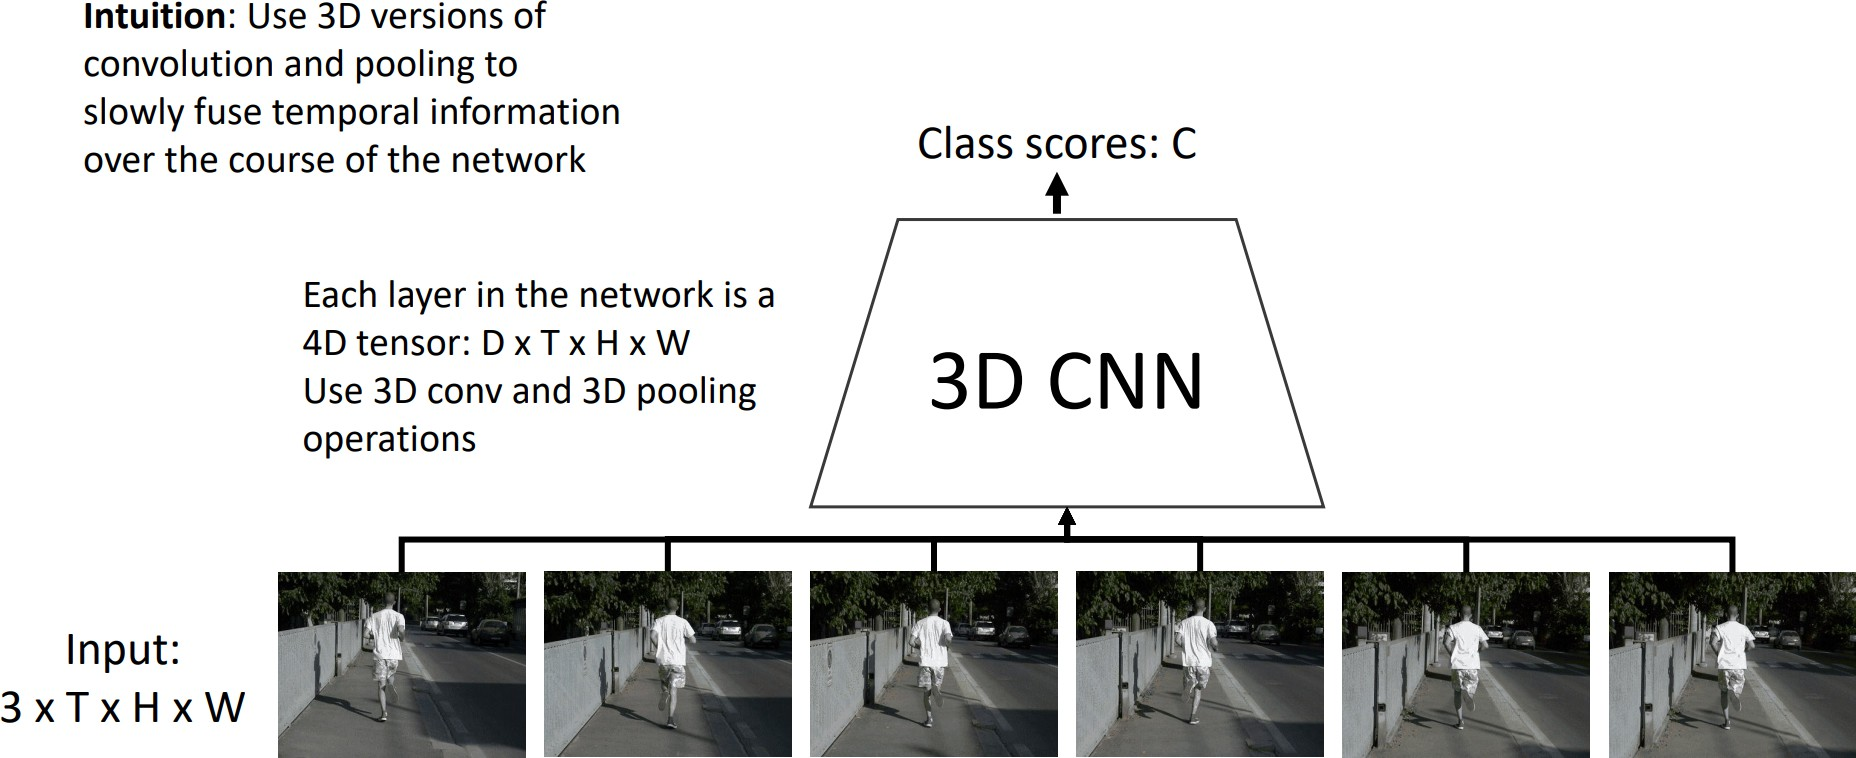
\includegraphics[width=1\textwidth,height=0.9\textheight,keepaspectratio]{images/video/slide_15_1_img.jpg}
    \end{figure}
\framebreak
    \begin{figure}
        \centering
        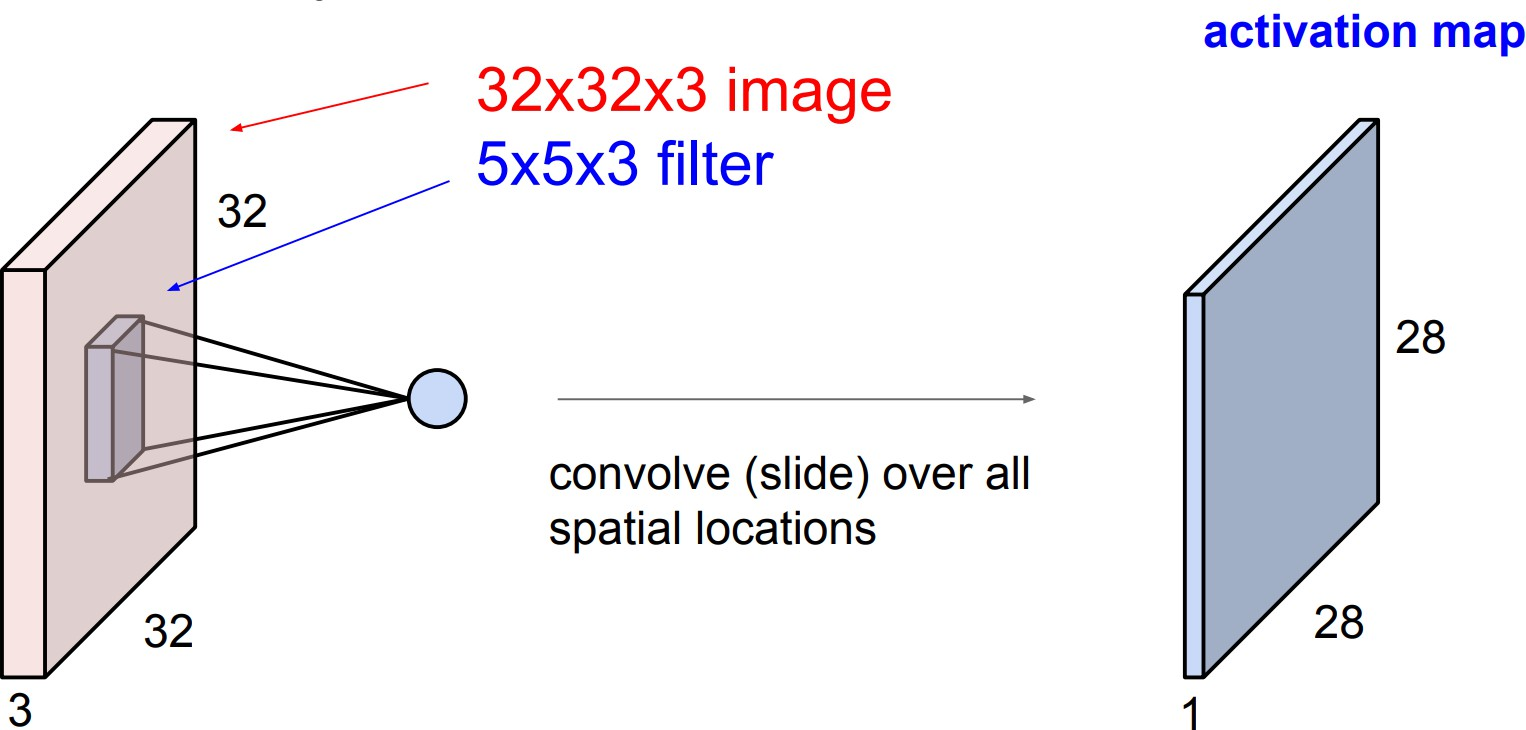
\includegraphics[width=1\textwidth,height=0.9\textheight,keepaspectratio]{images/video/slide_16_1_img.jpg}
    \end{figure}
\framebreak
    \begin{figure}
        \centering
        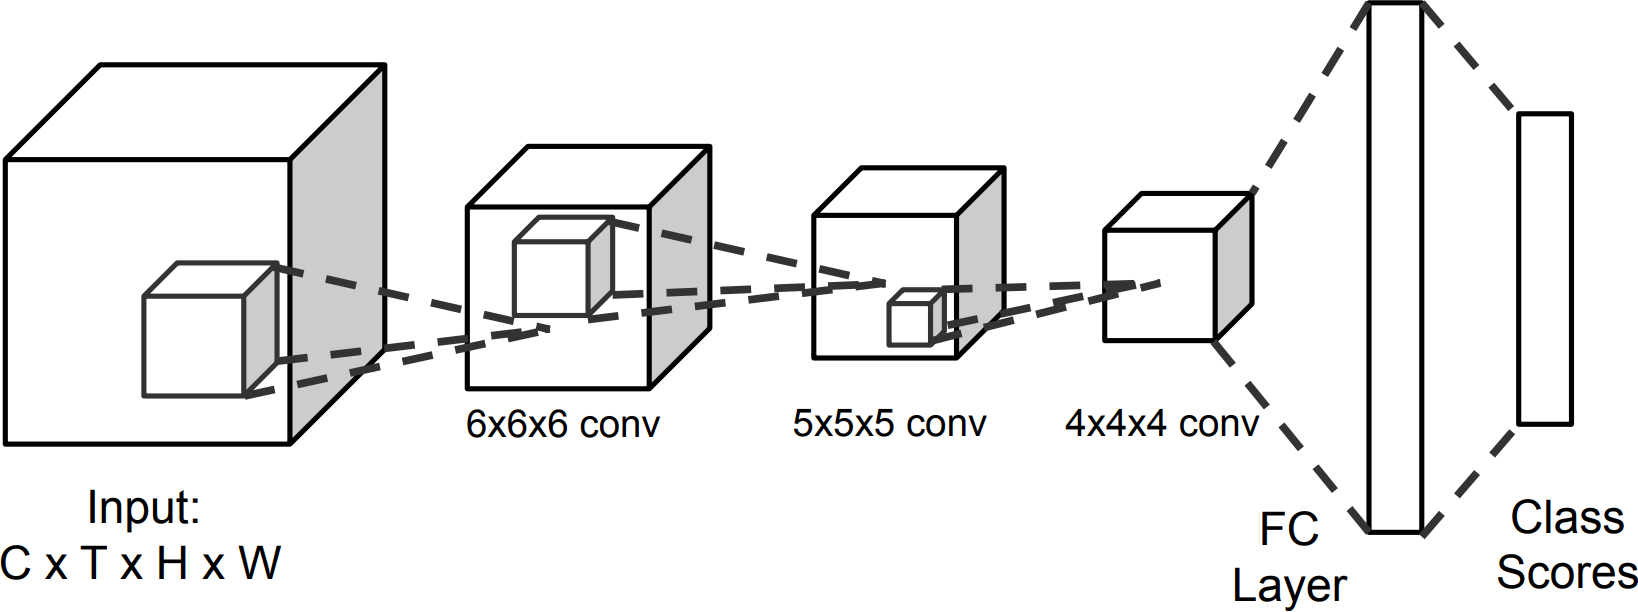
\includegraphics[width=1\textwidth,height=0.9\textheight,keepaspectratio]{images/video/slide_17_1_img.png}
    \end{figure}
\framebreak
    \begin{itemize}
        \item \textbf{3D CNNs} are powerful for video understanding, capturing both spatial and temporal features.
        \item They are particularly effective for tasks like action recognition, where understanding motion is crucial.
        \item However, they require significant computational resources and large datasets for training.
        \item \textbf{Applications}:
        \begin{itemize}
            \item Action recognition in videos.
            \item Gesture recognition.
            \item Video classification.
            \item Sports analysis.
        \end{itemize}
    \end{itemize}
\end{frame}